
\section{Das Relativitätsprinzip 
\label{relativ:section:relativistik}}
\rhead{Das Relativitätsprinzip}

Um relativistische Mechanik verstehen zu können,
muss natürlich zuerst auf das Relativitätsprinzip eingegangen werden.
Dabei gibt es zwei wesentliche Unterschiede zur klassischen Mechanik.

Der erste wichtige Unterschied ist, dass die Zeit unter relativistischer Betrachtung keine absolute Grösse mehr ist.
Geschehenes kann also nicht einfach anhand eines starren Zeitstrahls erklärt werden, sondern die Zeit ist abhängig vom Betrachter.
Man geht über vom dreidimensionalen Raum in die vierdimensionale Raumzeit, in welcher die Welt relativistisch beschrieben wird.

Der zweite Unterschied ist,
dass die Geschwindigkeit der Wirkungsausbreitung begrenzt ist,
und zwar durch die Lichtgeschwindigkeit
\(c=299792458\unit[per-mode = fraction]{\metre\per\second}\).
Diese ist zwar auch in der klassischen Mechanik eine Konstante,
jedoch ist die Geschwindigkeit der Wirkungsausbreitung dort unbegrenzt.
Ein einfaches Beispiel, um dies zu veranschaulichen,
ist die Betrachtung von starren Körpern in der klassischen Mechanik.
Wird ein starrer Körper beispielsweise an einem Punkt angestossen,
so muss sich, gemäss Definition eines starren Körpers,
jeder Teil dieses Körpers augenblicklich und zeitgleich in Bewegung setzen.
Dies bedeutet also, dass sich die Wirkung (Anstossen des Körpers)
vom Punkt aus, in dem dieser angestossen wurde,
mit unendlicher Geschwindigkeit in alle Teile des Körpers ausbreitet.


\subsection{Koordinatentransformationen 
\label{relativ:section:koordtrafo}}

Koordinatentransformationen werden benutzt,
um Koordinaten aus einem Bezugssystem in diejenigen eines anderen Bezugssystems umzurechnen.
In der Physik dienen sie beispielsweise dazu,
ein System oder einen Vorgang aus einer anderen Perspektive bzw.
von einem anderen Referenzpunkt aus zu beschreiben.

\subsubsection{Galilei-Transformation 
\label{relativ:section:galilei-trafo}}

In der klassischen Mechanik gibt es die folgenden,
intuitiven Transformationen, um zwischen verschiedenen Bezugssystemen
zu vergleichen:
\[
\begin{aligned}
    &\text{Translation in der Zeit: } && t \rightarrow t + b \\
    &\text{Translation im Raum: } && \vec{r} \rightarrow \vec{r} + \vec{a} \\
    &\text{Orthogonale Drehung: } && \vec{r} \rightarrow A \vec{r} \\
    &\text{Transformation auf ein Bezugssystem mit Relativgeschwindigkeit: } && \vec{r} \rightarrow \vec{r} + \vec{v} \cdot t .
\end{aligned}
\]
Eine Kombination aus diesen Transformationen wird als Galilei-Transformation bezeichnet.
Ein einfaches Beispiel dafür ist in Abbildung~\ref{relativ:fig:galilei-trafo} zu finden.
\begin{figure}
    \centering
    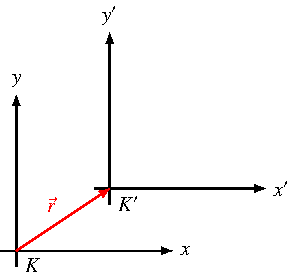
\includegraphics{papers/relativ/tikz/galilei_trafo.pdf}
    \caption{Darstellung einer einfachen Galilei-Transformation in \(\mathbb{R}^2\)
    vom Koordinatensystem \(K\) zum System \(K'\).
    Sie besteht lediglich aus einer Translation um den Vektor \(\vec{r}\).
    \label{relativ:fig:galilei-trafo}}
\end{figure}

\subsubsection{Lorentz-Transformation 
\label{relativ:section:lorentz-trafo}}

In der relativistischen Mechanik muss man sich hingegen der Lorentz-Transformation bedienen,
welche eine Erweiterung der Galilei-Transformation darstellt
und wesentlich kompliziertere Formeln annehmen kann.
Beispielsweise ergeben sich die Transformation von einem
Bezugssystem \(K\) in ein anderes System \(K'\),
welches sich entlang der \(x\)-Achse mit der Geschwindigkeit \(V\)
relativ zu \(K\) bewegt (siehe Abbildung~\ref{relativ:fig:lorentz-trafo-koords}),
die Gleichungen
\begin{equation}
    x = \frac{x' + V t'}{\sqrt{1 - \frac{V^2}{c^2}}}, \quad
    y = y', \quad
    z = z', \quad
    t = \frac{t' + \frac{V}{c^2}x'}{\sqrt{1-\frac{V^2}{c^2}}}.
    \label{relativ:eqn:lorentz-trafo-beisp}
\end{equation}
\begin{figure}
    \centering
    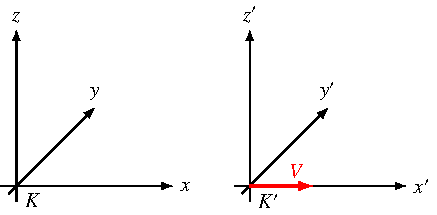
\includegraphics{papers/relativ/tikz/lorentz-trafo-koord.pdf}
    \caption{Bezugssystem \(K\) und ein zweites Koordinatensystem \(K'\),
    welches sich relativ zu \(K\) mit der konstanten Geschwindigkeit \(V\)
    entlang der \(x\)-Achse bewegt.
    \label{relativ:fig:lorentz-trafo-koords}}
\end{figure}

\subsection{Der Abstand 
\label{relativ:section:abstand}}

Ebenfalls muss der Begriff des Abstands für die relativistische Mechanik umformuliert werden.
In der klassischen Mechanik ist der euklidische Abstand
\begin{equation}
    ds=\sqrt{dx^2 + dy^2 + dz^2}
    \label{relativ:eqn:abstand-klass}
\end{equation}
für alle Bezugssysteme identisch.

Analog dazu gibt es in der relativistischen Mechanik den erweiterten Abstand
\begin{equation}
    ds = \sqrt{c^2dt^2 - dx^2 - dy^2 - dz^2},
    \label{relativ:eqn:abstand-relativ}
\end{equation}
welcher ebenfalls für verschiedene Bezugssysteme identisch ist.


\subsection{Die Eigenzeit 
\label{relativ:section:eigenzeit}}

Angenommen, wir beobachten eine Uhr,
welche sich in unserem Koordinatensystem um die Strecke
\(\sqrt{dx^2 + dy^2 + dz^2}\)
bewegt.
Im Koordinatensystem der Uhr gilt
\(dx' = dy' = dz' = 0\).
Gemäss der Invarianz des Abstands gilt somit
\begin{equation*}
    \underbrace{ds^2 = c^2 dt^2 - dx^2 - dy^2 - dz^2}_{\text{Unser Koordinatensystem}}
        = \underbrace{ds'^2 = c^2 dt'^2}_{\text{Koordinatensystem der Uhr}} .
\end{equation*}
Wird dieser Ausdruck nach dem Differential der Zeit im System der Uhr aufgelöst,
so folgt
\begin{equation}
    dt' = \frac{ds}{c} = \frac{ds'}{c}
    = dt \sqrt{1 - \frac{dx^2+dy^2+dz^2}{c^2 dt^2}}
    = dt \sqrt{1 - \frac{v^2}{c^2}}.
    \label{relativ:eqn:differential-eigenzeit}
\end{equation}
Dieses Zeitdifferential kann nun zur Zeitdifferenz
\begin{equation}
    t_2' - t_1' = \int_{t_1}^{t_2} dt \sqrt{1 - \frac{v^2}{c^2}}
    \label{relativ:eqn:eigenzeit}
\end{equation}
integriert werden.
Das ist nun die Zeit, die von der bewegten Uhr gemessen wird.
Eine solche Zeit, welche von einer Uhr,
welche sich mit einem Gegenstand mitbewegt, gemessen wird,
nennt man \emph{Eigenzeit}.
Durch den Ausdruck unter der Wurzel wird auch klar,
dass die Zeitdifferenz \(t_2'- t_1'\) kleiner ist
als \(t_2 - t_1\) im Referenzsystem.
Daher kommt auch der Ausdruck
``bewegte Uhren gehen langsamer''.
